\documentclass{standalone}
\usepackage{tikz}
\usetikzlibrary{patterns, positioning}

\begin{document}
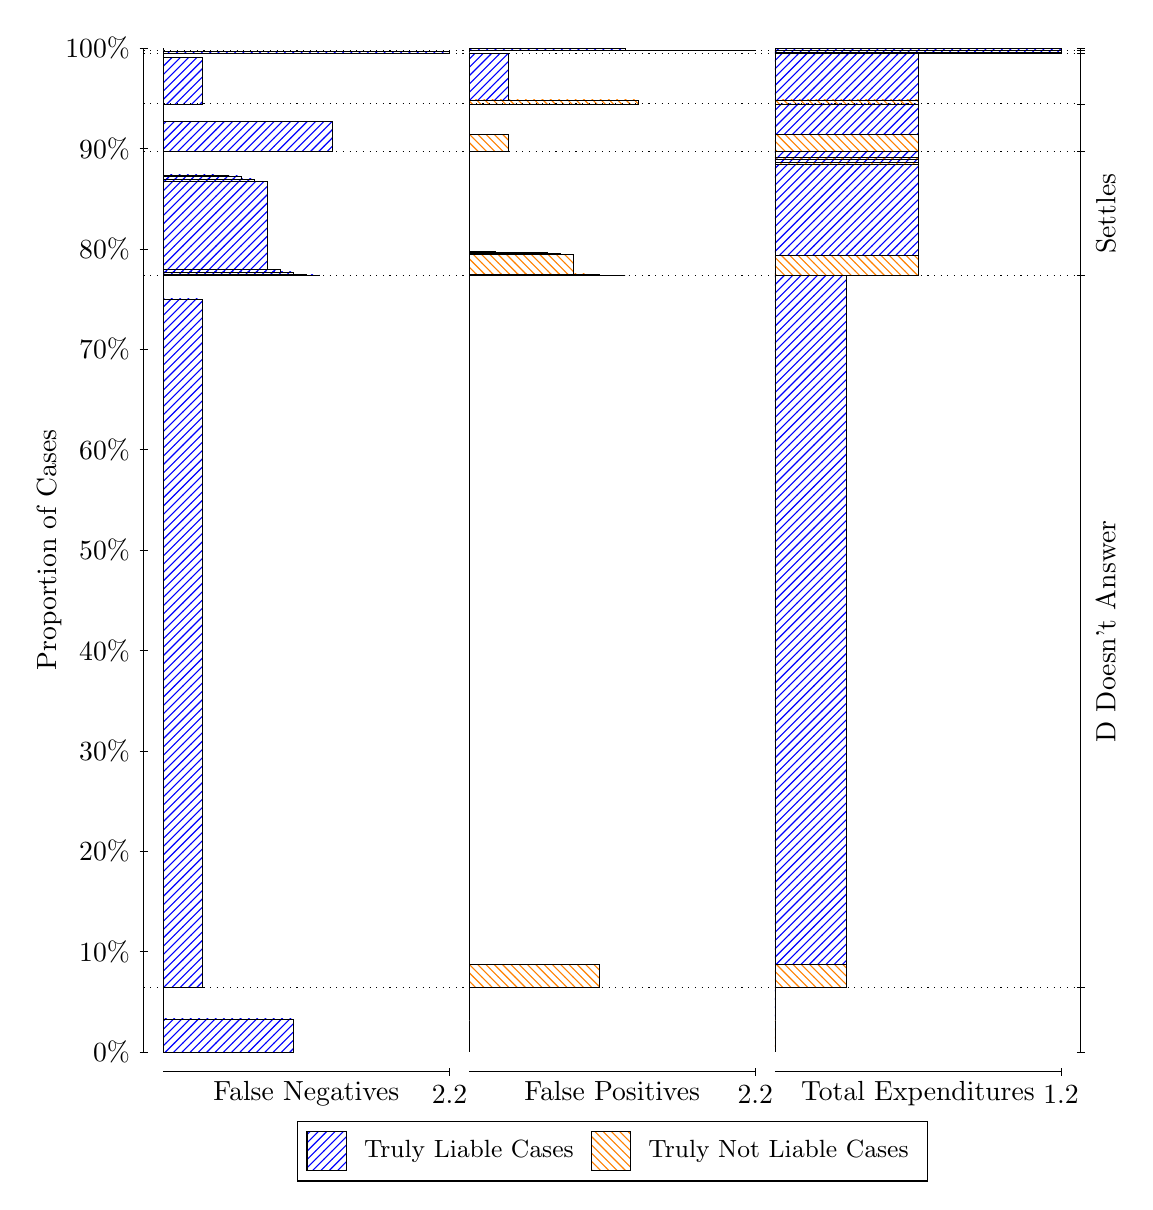
\begin{tikzpicture}
\draw[black, very thin] (1.5,1.75) -- (1.5,14.5);
\node[rotate=90, anchor=center] at (0.3, 8.125) {Proportion of Cases};
\draw[black, very thin] (1.45,1.75) -- (1.55,1.75);
\node[anchor=east] at (1.45, 1.75) {0\%};
\draw[black, very thin] (1.45,3.025) -- (1.55,3.025);
\node[anchor=east] at (1.45, 3.025) {10\%};
\draw[black, very thin] (1.45,4.3) -- (1.55,4.3);
\node[anchor=east] at (1.45, 4.3) {20\%};
\draw[black, very thin] (1.45,5.575) -- (1.55,5.575);
\node[anchor=east] at (1.45, 5.575) {30\%};
\draw[black, very thin] (1.45,6.85) -- (1.55,6.85);
\node[anchor=east] at (1.45, 6.85) {40\%};
\draw[black, very thin] (1.45,8.125) -- (1.55,8.125);
\node[anchor=east] at (1.45, 8.125) {50\%};
\draw[black, very thin] (1.45,9.4) -- (1.55,9.4);
\node[anchor=east] at (1.45, 9.4) {60\%};
\draw[black, very thin] (1.45,10.675) -- (1.55,10.675);
\node[anchor=east] at (1.45, 10.675) {70\%};
\draw[black, very thin] (1.45,11.95) -- (1.55,11.95);
\node[anchor=east] at (1.45, 11.95) {80\%};
\draw[black, very thin] (1.45,13.225) -- (1.55,13.225);
\node[anchor=east] at (1.45, 13.225) {90\%};
\draw[black, very thin] (1.45,14.5) -- (1.55,14.5);
\node[anchor=east] at (1.45, 14.5) {100\%};

\draw[black, very thin] (13.4,1.75) -- (13.4,14.5);
\draw[black, very thin] (13.35,1.75) -- (13.45,1.75);
\node[anchor=west] at (13.35, 1.75) {};
\draw[black, very thin] (13.35,2.5694) -- (13.45,2.5694);
\node[anchor=west] at (13.35, 2.5694) {};
\draw[black, very thin] (13.35,11.611) -- (13.45,11.611);
\node[anchor=west] at (13.35, 11.611) {};
\draw[black, very thin] (13.35,13.184) -- (13.45,13.184);
\node[anchor=west] at (13.35, 13.184) {};
\draw[black, very thin] (13.35,13.79) -- (13.45,13.79);
\node[anchor=west] at (13.35, 13.79) {};
\draw[black, very thin] (13.35,14.433) -- (13.45,14.433);
\node[anchor=west] at (13.35, 14.433) {};
\draw[black, very thin] (13.35,14.469) -- (13.45,14.469);
\node[anchor=west] at (13.35, 14.469) {};
\draw[black, very thin] (13.35,14.5) -- (13.45,14.5);
\node[anchor=west] at (13.35, 14.5) {};

\draw[black, very thin, pattern color=blue, pattern=north east lines] (1.75,1.75) rectangle (3.4015,2.1713);
\draw[black, very thin, pattern color=orange, pattern=north west lines] (1.75,2.1713) rectangle (1.75,2.5694);
\draw[black, very thin, pattern color=blue, pattern=north east lines] (1.75,2.5694) rectangle (2.2455,11.313);
\draw[black, very thin, pattern color=orange, pattern=north west lines] (1.75,11.313) rectangle (1.75,11.611);
\draw[black, very thin, pattern color=blue, pattern=north east lines] (1.75,11.611) rectangle (3.7318,11.619);
\draw[black, very thin, pattern color=blue, pattern=north east lines] (1.75,11.619) rectangle (3.5667,11.622);
\draw[black, very thin, pattern color=blue, pattern=north east lines] (1.75,11.622) rectangle (3.4015,11.657);
\draw[black, very thin, pattern color=blue, pattern=north east lines] (1.75,11.657) rectangle (3.2364,11.657);
\draw[black, very thin, pattern color=blue, pattern=north east lines] (1.75,11.657) rectangle (3.2364,11.69);
\draw[black, very thin, pattern color=blue, pattern=north east lines] (1.75,11.69) rectangle (3.0712,12.808);
\draw[black, very thin, pattern color=blue, pattern=north east lines] (1.75,12.808) rectangle (2.9061,12.839);
\draw[black, very thin, pattern color=blue, pattern=north east lines] (1.75,12.839) rectangle (2.7409,12.875);
\draw[black, very thin, pattern color=blue, pattern=north east lines] (1.75,12.875) rectangle (2.5758,12.88);
\draw[black, very thin, pattern color=blue, pattern=north east lines] (1.75,12.88) rectangle (2.4106,12.888);
\draw[black, very thin, pattern color=orange, pattern=north west lines] (1.75,12.888) rectangle (1.75,13.184);
\draw[black, very thin, pattern color=blue, pattern=north east lines] (1.75,13.184) rectangle (3.897,13.571);
\draw[black, very thin, pattern color=orange, pattern=north west lines] (1.75,13.571) rectangle (1.75,13.79);
\draw[black, very thin, pattern color=blue, pattern=north east lines] (1.75,13.79) rectangle (2.2455,14.383);
\draw[black, very thin, pattern color=orange, pattern=north west lines] (1.75,14.383) rectangle (1.75,14.433);
\draw[black, very thin, pattern color=blue, pattern=north east lines] (1.75,14.433) rectangle (5.3833,14.456);
\draw[black, very thin, pattern color=orange, pattern=north west lines] (1.75,14.456) rectangle (1.75,14.469);
\draw[black, very thin, pattern color=orange, pattern=north west lines] (1.75,14.469) rectangle (1.75,14.471);
\draw[black, very thin, pattern color=blue, pattern=north east lines] (1.75,14.471) rectangle (1.75,14.5);
\draw[black, very thin, pattern color=orange, pattern=north west lines] (5.6333,1.75) rectangle (5.6333,2.1481);
\draw[black, very thin, pattern color=blue, pattern=north east lines] (5.6333,2.1481) rectangle (5.6333,2.5694);
\draw[black, very thin, pattern color=orange, pattern=north west lines] (5.6333,2.5694) rectangle (7.2848,2.8666);
\draw[black, very thin, pattern color=blue, pattern=north east lines] (5.6333,2.8666) rectangle (5.6333,11.611);
\draw[black, very thin, pattern color=orange, pattern=north west lines] (5.6333,11.611) rectangle (7.6152,11.611);
\draw[black, very thin, pattern color=orange, pattern=north west lines] (5.6333,11.611) rectangle (7.45,11.612);
\draw[black, very thin, pattern color=orange, pattern=north west lines] (5.6333,11.612) rectangle (7.2848,11.622);
\draw[black, very thin, pattern color=orange, pattern=north west lines] (5.6333,11.622) rectangle (7.1197,11.632);
\draw[black, very thin, pattern color=orange, pattern=north west lines] (5.6333,11.632) rectangle (6.9545,11.878);
\draw[black, very thin, pattern color=orange, pattern=north west lines] (5.6333,11.878) rectangle (6.7894,11.889);
\draw[black, very thin, pattern color=orange, pattern=north west lines] (5.6333,11.889) rectangle (6.6242,11.9);
\draw[black, very thin, pattern color=orange, pattern=north west lines] (5.6333,11.9) rectangle (6.4591,11.901);
\draw[black, very thin, pattern color=orange, pattern=north west lines] (5.6333,11.901) rectangle (6.2939,11.907);
\draw[black, very thin, pattern color=blue, pattern=north east lines] (5.6333,11.907) rectangle (5.9636,11.914);
\draw[black, very thin, pattern color=blue, pattern=north east lines] (5.6333,11.914) rectangle (5.7985,11.919);
\draw[black, very thin, pattern color=blue, pattern=north east lines] (5.6333,11.919) rectangle (5.6333,13.184);
\draw[black, very thin, pattern color=orange, pattern=north west lines] (5.6333,13.184) rectangle (6.1288,13.403);
\draw[black, very thin, pattern color=blue, pattern=north east lines] (5.6333,13.403) rectangle (5.6333,13.79);
\draw[black, very thin, pattern color=orange, pattern=north west lines] (5.6333,13.79) rectangle (7.7803,13.84);
\draw[black, very thin, pattern color=blue, pattern=north east lines] (5.6333,13.84) rectangle (6.1288,14.433);
\draw[black, very thin, pattern color=orange, pattern=north west lines] (5.6333,14.433) rectangle (5.6333,14.446);
\draw[black, very thin, pattern color=blue, pattern=north east lines] (5.6333,14.446) rectangle (5.6333,14.469);
\draw[black, very thin, pattern color=orange, pattern=north west lines] (5.6333,14.469) rectangle (9.2667,14.471);
\draw[black, very thin, pattern color=blue, pattern=north east lines] (5.6333,14.471) rectangle (7.6152,14.5);
\draw[black, very thin, pattern color=orange, pattern=north west lines] (9.5167,1.75) rectangle (9.5167,2.1481);
\draw[black, very thin, pattern color=blue, pattern=north east lines] (9.5167,2.1481) rectangle (9.5167,2.5694);
\draw[black, very thin, pattern color=orange, pattern=north west lines] (9.5167,2.5694) rectangle (10.425,2.8666);
\draw[black, very thin, pattern color=blue, pattern=north east lines] (9.5167,2.8666) rectangle (10.425,11.611);
\draw[black, very thin, pattern color=orange, pattern=north west lines] (9.5167,11.611) rectangle (11.333,11.868);
\draw[black, very thin, pattern color=blue, pattern=north east lines] (9.5167,11.868) rectangle (11.333,13.027);
\draw[black, very thin, pattern color=orange, pattern=north west lines] (9.5167,13.027) rectangle (11.333,13.045);
\draw[black, very thin, pattern color=blue, pattern=north east lines] (9.5167,13.045) rectangle (11.333,13.092);
\draw[black, very thin, pattern color=orange, pattern=north west lines] (9.5167,13.092) rectangle (11.333,13.113);
\draw[black, very thin, pattern color=blue, pattern=north east lines] (9.5167,13.113) rectangle (11.333,13.184);
\draw[black, very thin, pattern color=orange, pattern=north west lines] (9.5167,13.184) rectangle (11.333,13.403);
\draw[black, very thin, pattern color=blue, pattern=north east lines] (9.5167,13.403) rectangle (11.333,13.79);
\draw[black, very thin, pattern color=orange, pattern=north west lines] (9.5167,13.79) rectangle (11.333,13.84);
\draw[black, very thin, pattern color=blue, pattern=north east lines] (9.5167,13.84) rectangle (11.333,14.433);
\draw[black, very thin, pattern color=orange, pattern=north west lines] (9.5167,14.433) rectangle (13.15,14.446);
\draw[black, very thin, pattern color=blue, pattern=north east lines] (9.5167,14.446) rectangle (13.15,14.469);
\draw[black, very thin, pattern color=orange, pattern=north west lines] (9.5167,14.469) rectangle (13.15,14.471);
\draw[black, very thin, pattern color=blue, pattern=north east lines] (9.5167,14.471) rectangle (13.15,14.5);
\draw[black, dotted] (1.5,2.5694) -- (13.4,2.5694);
\draw[black, dotted] (1.5,11.611) -- (13.4,11.611);
\draw[black, dotted] (1.5,13.184) -- (13.4,13.184);
\draw[black, dotted] (1.5,13.79) -- (13.4,13.79);
\draw[black, dotted] (1.5,14.433) -- (13.4,14.433);
\draw[black, dotted] (1.5,14.469) -- (13.4,14.469);
\draw[black, very thin] (1.75,1.5) -- (5.3833,1.5);
\node[anchor=north] at (3.5667, 1.5) {False Negatives};
\draw[black, very thin] (5.3833,1.45) -- (5.3833,1.55);
\node[anchor=north] at (5.3833, 1.45) {2.2};

\draw[black, very thin] (5.6333,1.5) -- (9.2667,1.5);
\node[anchor=north] at (7.45, 1.5) {False Positives};
\draw[black, very thin] (9.2667,1.45) -- (9.2667,1.55);
\node[anchor=north] at (9.2667, 1.45) {2.2};

\draw[black, very thin] (9.5167,1.5) -- (13.15,1.5);
\node[anchor=north] at (11.333, 1.5) {Total Expenditures};
\draw[black, very thin] (13.15,1.45) -- (13.15,1.55);
\node[anchor=north] at (13.15, 1.45) {1.2};


\node[black, centered, rotate=90] at (13.72, 7.09) {D Doesn't Answer};
\node[black, centered, rotate=90] at (13.72, 12.397) {Settles};





\draw (7.449999999999999,1.5) node[draw=none] (baseCoordinate) {};
\begin{scope}[align=center]
        \matrix[scale=0.5, draw=black, below=0.5cm of baseCoordinate, nodes={draw}, column sep=0.1cm]{
            \node[rectangle, draw, minimum width=0.5cm, minimum height=0.5cm, pattern=north east lines, pattern color=blue] {}; &
            \node[draw=none, font=\small] (B) {Truly Liable Cases}; &
            \node[rectangle, draw, minimum width=0.5cm, minimum height=0.5cm, pattern=north west lines, pattern color=orange] {}; &
            \node[draw=none, font=\small] (B) {Truly Not Liable Cases}; \\
            };
\end{scope}

\end{tikzpicture}
\end{document}